Para la realización de este trabajo se ha utilizado un conjunto de datos que se ha creado aleatoriamente. 

El conjunto de datos lo conforma un grafo no dirigido con pesos en sus aristas. El número de nodos es 10.

El grafo se crea a partir de un fichero \textit{CSV} que contiene los datos siguientes:

\begin{center}
	\begin{tabular}{ |c|c| } 
		(u, v) & w \\ 
		\hline
		(0,1) & 3 \\
		(0,4) & 10 \\
		(0,5) & 2 \\
		(1,2) & 5 \\
		(1,6) & 2 \\
		(2,3) & 8 \\
		(2,7) & 8 \\
		(3,8) & 8 \\
		(3,4) & 7 \\
		(4,5) & 4 \\
		(4,8) & 2 \\
		(4,9) & 8 \\
		(5,7) & 1 \\
		(6,8) & 7 \\
		(6,9) & 7 \\
		(7,9) & 10 \\
		\hline
	\end{tabular}
\end{center}

\begin{center}
	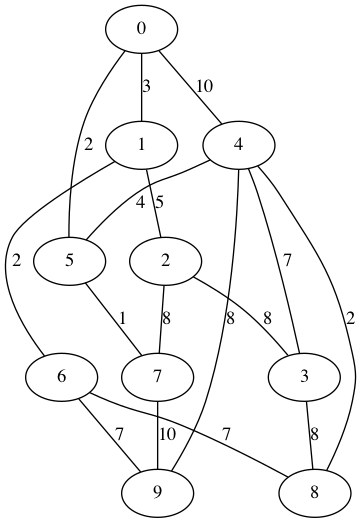
\includegraphics[scale=0.5]{../dataset/dataset}
\end{center}